\subsection{Prototype 1 [JG]}

The fridge has become an essential product in almost any kitchen since its invention.
As a result, the main ideas behind its design have been refined to a point of near perfection, leaving little room for innovation, and even less for improvement.
Therefore, the challenge when designing the Smart Fridge did not come from trying to change or improve an established design, but rather came from implementing new features whilst staying as close to this design as possible.

The Smart Fridge would take the form of a box which would be large enough to fit a small bottle of milk inside.
The ESP camera was to be fitted into the door.
Initially, it was decided that the door would be thick and hollow to store the camera and the electrical components associated with it.
The door would also house the Hall effect sensor to detect whether the fridge door was open.
The weight sensor was then to be placed on the bottom of the fridge, with a plate above it on which items would be placed.
The remaining electrical components would then be placed in this gap.
For the prototype it was decided that this would remain open for easier access should any changes need to be made.
The CAD design for this is shown below with dimensions.

\begin{figure}[H]        
    \centering
    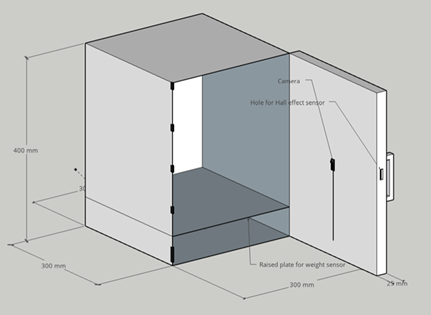
\includegraphics[width=.33\textwidth]{Chapter 5/Box/BoxSchematic1.png}
    \caption{Initial design of Smart Fridge.}
    \label{fig:initaldesign}
\end{figure} 

The biggest issue with this design was its size.
The dimensions of the box were 300mmx300mmx400mm in addition to the door which was 300mmx25mmx400mm.
 Therefore, it is likely that this design would have required 4 sheets of acrylic to build which would have been too expensive.
As a result, a new design was proposed with a smaller size.
These changes along with the new dimensions are shown below.

\begin{figure}[H]        
    \centering
    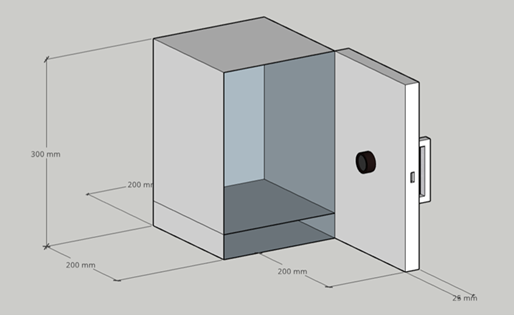
\includegraphics[width=.33\textwidth]{Chapter 5/Box/BoxSchematic2.png}
    \caption{Updated Fridge Design.}
    \label{fig:updatedfridge}
\end{figure} 


In figure 2 the dimensions of the main box were all reduced by 100mm, with the relevant changes also being applied to the dimensions of the door.
Figure 2 also shows the change from the ESP camera to a webcam, which now protrudes significantly from the door.
The webcam also has a much larger cross-sectional area with a diameter of around 33mm.
Despite these changes, the design was still too big, so a new design was proposed.
This is shown below.

\begin{figure}[H]        
    \centering
    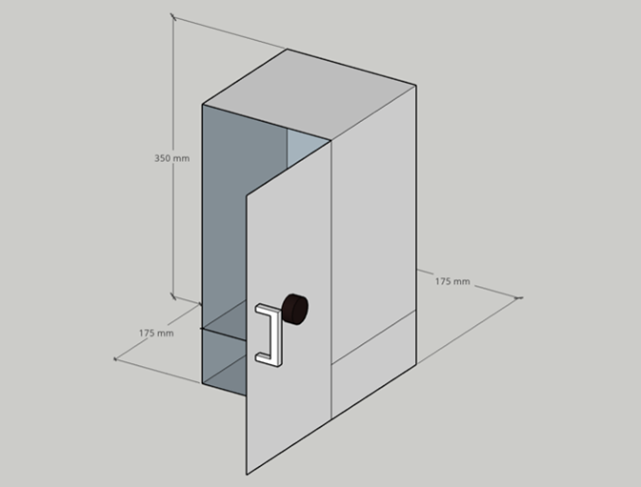
\includegraphics[width=.33\textwidth]{Chapter 5/Box/Schematic2DoorOpen.png}
    \caption{Fridge Design using 2 acrylic sheets.}
    \label{fig:fridge2sheet}
\end{figure} 

Figure 3 shows the changes made to the previous box design.
These changes reduced the required acrylic sheets from 3 to 2.
Firstly, the dimensions of the box were changed in order to achieve the maximum size possible while using no more than 2 acrylic sheets.
As a result, the dimensions of the base of the box were decreased, whilst the height was increased.
Previously it had been decided that the door would be a separate, thinner box.
However, to save acrylic, it was necessary for the door to be flat.
As a result, the components that would have previously been stored within the door now had to be stored under the weight sensor plate.
This meant that the weight sensor plate had to be raised by a few centimetres.
This box was then built with the final product shown below.

\begin{figure}[H]        
    \centering
    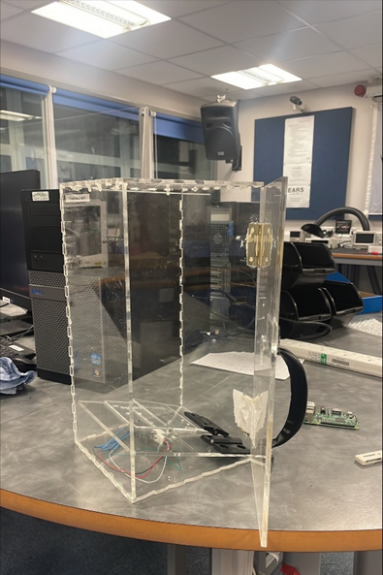
\includegraphics[width=.33\textwidth]{Chapter 5/Box/PictureOfBox1.png}
    \caption{First Built Box}
    \label{fig:firstbuilt}
\end{figure} 

There were several issues with the proposed design in figure 4.
The most noticeable of these issues is the collapsed weight sensor plate inside the box.
This happened as too much space was given on each side to ensure it would fit.
The other main problem with the box was that gluing objects onto acrylic was difficult.
This was especially true of the side plates and the door where objects had to be glued on vertically and would sometimes slide down.
This caused further problems with the hinges as they did not remain in their exact positions when stuck.
The hinges also did not allow the door to close entirely, leaving a small yet significant gap between the door and the box.
As a result, many aspects of the box had to be redesigned which led to a new proposal for the box design.
This is shown in the image below.

\begin{figure}[H]        
    \centering
    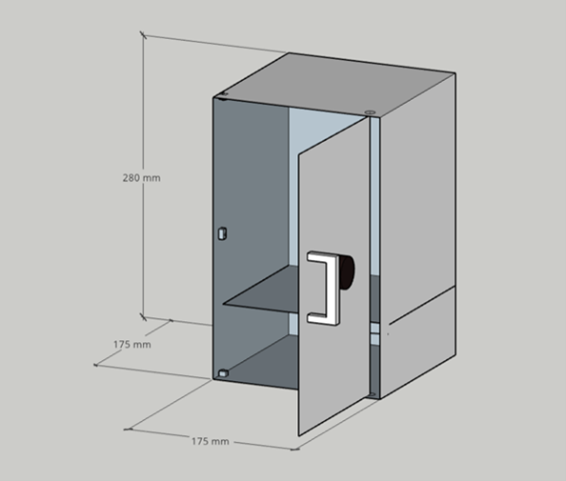
\includegraphics[width=.33\textwidth]{Chapter 5/Box/BoxDesign3.png}
    \caption{Fridge Design with no Hinges}
    \label{fig:designnohinges}
\end{figure} 

When designing the new box, shown in figure 5, the main idea was to remove the need for glue.
For the hinges, this was achieved by making a small hole in both the top and bottom plates of the box.
Then a single tooth was added onto the corresponding sides of the door to fit through these holes.
This also removed the need to use hinges which caused issues when closing the door in the previous design.
However, this meant that the door, now inside the box, would close in on itself.
To prevent this from happening, it was decided that small pieces of acrylic could be placed to act as door stoppers.
Each of these would be held in place by a single screw.
Additionally, the outward facing edge of the weight sensor plate had to be moved back into the fridge in order to avoid collisions with the door.
There was also a reduction in the height of the box as the previous design felt disproportionately tall.
Small changes were also made to the way in which the door handle was held in place.
In this design, holes were cut into the door for the two ends of the handle to be more securely attached.

\subsection{Prototype 2 [YJ]}

The box design for prototype 2 was the second iteration designed to make the box more user-friendly and fix the previous issues that prototype 1 encumbered.
However, facing concerns with a small budget, the containment would continue to use single-layer pieces of acrylic sheets.

The containment for the brains of the Smart-Fridge is below the main visible user body allowing easy access to the board by uncapping the bottom plate.
The magnets that detect when the door is open now mimic a soft closing door is a standard in most modern expensive fridges.
Magnets glued inside engravings allow for direct non-contact magnetic snapping to each other when the door is closed.
The plate onto which the Load cell and the Motherboard also use magnets to keep the platform intact.

The new design has no extra protrusions except for the camera.
There is simplistic cable management using zip ties.
The hinges from the first build-in prototype one secured through screws and nuts rather than glue resulting in a secure design as the hinges before were not firm and kept falling.
The redesign of the door handle resulted in curved edges rather than sharp which were previously not user-friendly and could have been harmful to the user.